% eq:E.2-PAW and eq:E.2-rhoPAW are second labels on eq:3.5-PAW and eq:3.5-rhoAE (amsmath allows one \label per equation, hence \ltx@label).
\section{Plane waves and the core region}\label{sec:3.5}

What a plane-wave code keeps, what a pseudopotential removes and how the projector-augmented-wave method puts it back decide the vertex at large $q$, together with the core states of silicon and germanium and the relativistic corrections that their electrons carry.

\subsection{Plane waves and the cutoff}

A plane-wave code stores each periodic part as the Fourier series \cref{eq:3.2-pw}, truncated to the reciprocal-lattice vectors inside a sphere,
\begin{equation}
  u_{n\vect{k}}(\vect{r}) = \frac{1}{\sqrt\Omega}\sum_{|\vect{k}+\vect{G}| \le k_{\mathrm{cut}}}c_{n\vect{k}}(\vect{G})\,\ee^{\ii\vect{G}\cdot\vect{r}}, \qquad
  E_{\mathrm{cut}} = \frac{k_{\mathrm{cut}}^2}{2m_e} .
  \label{eq:3.5-pw}
\end{equation}
The basis treats all regions of the cell alike and improves systematically as the cutoff $E_{\mathrm{cut}}$ is raised (\cref{app:E.1}). In \cref{eq:3.2-central} the kinetic energy is diagonal in $\vect{G}$, while the potential is diagonal in $\vect{r}$, and a fast Fourier transform between a grid of $\vect{G}$ and a grid of points in the cell applies each where it is diagonal. This is what makes plane waves the standard basis for crystals.

The price is paid near the nuclei. A state confined to a region of size $r_0$ has momentum components up to a few times $1/r_0$, and the innermost orbitals of an atom are small. A hydrogen-like $1s$ orbital of nuclear charge $Z$, $(p_0^3/\pi)^{1/2}\ee^{-p_0r}$ with $p_0 = Z\alpha m_e$, has the radius $1/p_0$. Its Fourier transform follows from $\int\dd^3r\,\ee^{-\ii\vect{p}\cdot\vect{r}}\ee^{-p_0r} = 8\pi p_0/(p^2 + p_0^2)^2$, and its momentum density, normalized to $\int\dd^3p = 1$, is $(8/\pi^2)\,p_0^5/(p^2 + p_0^2)^4$. For silicon, $p_0 = 14\times\SI{3.73}{keV} = \SI{52}{keV}$. Worse, the density falls as slowly as $p^{-8}$, a power law that comes from the cusp of the orbital at the nucleus, and so do the squared coefficients $|c_{n\vect{k}}(\vect{G})|^2$ of any state that has weight there. The valence states inherit a version of this tail. A $3s$ electron of silicon must be orthogonal to the $1s$ and $2s$ orbitals, and it does this by changing sign at 0.08 and \SI{0.38}{\angstrom} from the nucleus; a $3p$ electron changes sign at \SI{0.38}{\angstrom} to stay orthogonal to $2p$. These oscillations, and the cusp, are what a momentum transfer of tens of keV sees. To resolve the silicon $1s$ orbital alone, a plane-wave basis needs wavevectors up to a few times $Z/a_0$. With $3Z/a_0 = 42$ inverse bohr, \cref{eq:E.1-npw} asks for a cutoff near \SI{1800}{Ry} and $3\times10^5$ plane waves per state, 160 times the 2121 of the converged calculation of \cref{app:E.1}, and the cost of each band grows at least in proportion.

The vertex in plane waves is the sum \cref{eq:3.2-rhopw}. A term contributes only if both coefficients exist: the component $\vect{k}+\vect{G}$ of the initial state and the component $\vect{k}+\vect{G}+\vect{q}$ of the final state must both lie inside the cutoff sphere. Two points of a sphere of radius $k_{\mathrm{cut}}$ are at most $2k_{\mathrm{cut}}$ apart, and the computed vertex vanishes identically for $q > 2k_{\mathrm{cut}}$, which at \SI{60}{Ry} is \SI{58}{keV}. This bound would be reached if the two states had their weight at opposite ends of the sphere, and the kinematics of dark matter keeps them from it. By \cref{eq:1.3-vmin}, a momentum transfer $q$ deposits at most $\omega = qv_{\mathrm{max}}$, \SI{80}{eV} at $q = \SI{30}{keV}$, far below the free-electron energy $q^2/2m_e = \SI{0.88}{keV}$ at that momentum. The final state is a low-lying conduction state. Its plane-wave components are concentrated at momenta below a scale $p_f$ set by its energy above the bottom of the valence band, $p_f \simeq [2m_e(\omega + E_{\mathrm{F}})]^{1/2}$ with $E_{\mathrm{F}} = \SI{12.5}{eV}$ the free-electron value at the valence density (\cref{sec:2.5}). In \cref{eq:3.2-rhopw} the final-state coefficient at $\vect{k}+\vect{G}+\vect{q}$ is then appreciable for $|\vect{k}+\vect{G}+\vect{q}| \lesssim p_f$, and the initial state must supply the momentum, through its components at $|\vect{k}+\vect{G}| \simeq q$. The same holds with the two states exchanged. The vertex at momentum transfers up to $q_{\mathrm{max}}$ is converged once the basis contains these components,
\begin{equation}
  k_{\mathrm{cut}} \gtrsim q_{\mathrm{max}} + p_f, \qquad
  E_{\mathrm{cut}} \gtrsim \frac{(q_{\mathrm{max}} + p_f)^2}{2m_e} .
  \label{eq:3.5-Ecut}
\end{equation}
The large-$q$ vertex is the overlap of the high-momentum tail of one state with the low-momentum body of the other, as \cref{sec:3.2} anticipated. A cutoff converged for total energies says nothing about whether that tail is in the basis, and \cref{eq:3.5-Ecut} has to be checked separately for every rate calculation. Whether the tail is physical is another matter, which depends on the potential the states were computed in.

\subsection{Pseudopotentials}

The core electrons of silicon, $1s^2 2s^2 2p^6$, are bound by \SI{99}{eV} and more and take no part in bonding; their orbitals hardly change between the atom and the crystal. The valence electrons, however, feel them through orthogonality. A $3s$ state must be orthogonal to $1s$ and $2s$, and its two nodes inside \SI{0.4}{\angstrom} carry a large kinetic energy there. That kinetic energy acts like a repulsion that nearly cancels the attraction of the nucleus inside the core, and outside the core the valence electron sees a nucleus screened by ten electrons. Phillips and Kleinman made this precise: subtracting the core states from a valence state leaves a smooth function that obeys a Schr\"odinger equation with a weak, repulsive correction added to the potential inside the core~\cite{phillips1959new}. The cancellation is why the nearly-free-electron picture of \cref{sec:3.2} works for silicon at all, and why the empirical pseudopotential of \cref{sec:3.3} needs only three Fourier components.

A \emph{pseudopotential} turns the cancellation into a construction. It replaces the nucleus and the core electrons by an effective potential whose valence states are smooth and nodeless inside a \emph{core radius} $r_c$ and identical to the true, all-electron states outside it. The core states are dropped from the calculation, and with them the oscillations of the valence states that kept them orthogonal. The construction starts from an all-electron calculation of the atom and is carried out for each angular momentum $l$ separately. Hamann, Schl\"uter and Chiang formulated the conditions that make the result useful~\cite{hamann1979norm}. Two of them do the work. For a reference configuration of the atom, the pseudo and all-electron valence states must have the same eigenvalue and agree beyond $r_c$, and they must hold the same charge inside it. Their logarithmic derivatives at $r_c$ then agree, and so do the first energy derivatives of these. The charge condition, \emph{norm conservation}, is the one with content, and it implies the last.

To see this, write the radial Schr\"odinger equation for $u_l(r; \varepsilon) = rR_l(r)$ at energy $\varepsilon$ in a potential $V_l(r)$, which may differ from one $l$ to the next,
\begin{equation}
  -\frac{1}{2m_e}\,u_l'' + \Bigl[V_l(r) + \frac{l(l+1)}{2m_er^2} - \varepsilon\Bigr]u_l = 0 ,
  \label{eq:3.5-radial}
\end{equation}
with primes for $\partial/\partial r$, and differentiate it with respect to $\varepsilon$. The derivative $\dot u_l = \partial u_l/\partial\varepsilon$ obeys the same equation with the source $u_l$ on the right-hand side. Multiplying the equation for $u_l$ by $\dot u_l$, the equation for $\dot u_l$ by $u_l$, and subtracting, the potential drops out and leaves $(\dot u_lu_l' - u_l\dot u_l')' = 2m_eu_l^2$. Both functions vanish at the origin, and integrating to $r_c$,
\begin{equation}
  \frac{\partial}{\partial\varepsilon}\,\frac{u_l'(r_c)}{u_l(r_c)} = \frac{\dot u_l'u_l - u_l'\dot u_l}{u_l^2}\bigg|_{r_c} = -\frac{2m_e}{u_l(r_c)^2}\int_0^{r_c}\dd r\,u_l^2 .
  \label{eq:3.5-logder}
\end{equation}
The logarithmic derivative at $r_c$ fixes how a wave arriving from outside is scattered by everything inside, and \cref{eq:3.5-logder} ties its energy dependence to the charge inside the sphere. A pseudo-state that matches the all-electron state in value and slope at $r_c$ at the reference energy, and has the same charge inside, therefore scatters like the true atom to first order in the energy away from the reference. A potential fitted to the free atom then works in the crystal, where the valence energies are shifted by the bonding. Two or more reference energies per channel extend the range of energies over which it works. Vanderbilt introduced them in his ultrasoft scheme, which relaxes the norm-conservation condition of Hamann, Schl\"uter and Chiang and restores the missing charge with augmentation functions~\cite{vanderbilt1990soft}. Hamann's optimized potentials keep norm conservation in a generalized form: the overlaps $\int_0^{r_c}\dd r\,u_iu_j$ of the pseudo and all-electron reference states agree for every pair $i, j$~\cite[Eq.~(23)]{hamann2013optimized}.

The potential this produces is \emph{nonlocal}. Orthogonality acts only within one angular momentum: a $3s$ electron is pushed out by the $1s$ and $2s$ cores, a $3p$ electron by $2p$, and a $3d$ electron by nothing, since silicon has no $d$ core. The effective potential is then different in each channel, $\sum_lV_l(r)P_l$ with $P_l$ the projector on angular momentum $l$ about the nucleus, and in practice it is cast into a local part plus a few separable projections, the form \cref{eq:E.2-KB} of Kleinman and Bylander~\cite{kleinman1982efficacious}. A nonlocal potential does not commute with $\vect{r}$, and we have already met two consequences: the velocity is no longer $\vect{p}/m_e$ (\cref{sec:3.2}), and the $f$-sum rule acquires a correction (\cref{sec:4.3}). The density vertex needs none, since $\ee^{\ii\vect{q}\cdot\vect{r}}$ couples to the pseudo-states by multiplication, as in any Hamiltonian; its only error is the missing core region.

The core radius sets the trade-off. A large $r_c$ makes the pseudo-states smooth and the cutoff low, but asks one potential to describe a large part of the atom, and it transfers less well to other environments. The cutoff is decided by the Fourier tail of the pseudo-states, and the optimized construction of Hamann chooses the shape inside $r_c$ to minimize the kinetic energy above a wavevector $q_{\mathrm{opt}}$ (\cref{eq:E.2-residual}). In practice, the potentials of the plane-wave calculations of this book (\cref{app:E.1,app:E.2}) come from the SG15 library~\cite{schlipf2015optimization}. The silicon potential keeps the four $3s$ and $3p$ electrons, with $r_c = \SI{1.27}{\angstrom}$ for $s$ and \SI{1.89}{\angstrom} for $p$, and $q_{\mathrm{opt}} = 19$ and \SI{13}{keV}. With it, the total energy converges to \SI{0.1}{meV} per atom at about \SI{60}{Ry} (\cref{tab:E-cutoff}). \Cref{app:E.2} describes how such potentials are built and tested.

\Cref{fig:3-psae}(a) shows what is lost, for a norm-conserving silicon potential built with the SG15 core radii. The pseudo-orbitals agree with the all-electron ones beyond $r_c$ and are smooth and nodeless inside, where the true orbitals oscillate; the charge inside $r_c$ is the same, 0.662 of the $3s$ electron and 0.767 of the $3p$ electron. In momentum space, panel (b), the two agree to \SI{10}{\percent} below \SI{2}{keV} for $3s$ and \SI{5}{keV} for $3p$, where most of the weight is. Above, the pseudo-orbitals fall off much faster. Above \SI{10}{keV} the all-electron $3s$ orbital keeps \SI{7}{\percent} of its weight and the pseudo-orbital \SI{0.14}{\percent}; at \SI{30}{keV} the all-electron momentum densities exceed the pseudo ones by more than four orders of magnitude. A pseudopotential calculation converged in $E_{\mathrm{cut}}$ converges to the pseudo answer, and at large $q$ the pseudo answer is wrong.

\begin{figure}[tbp]
  \centering
  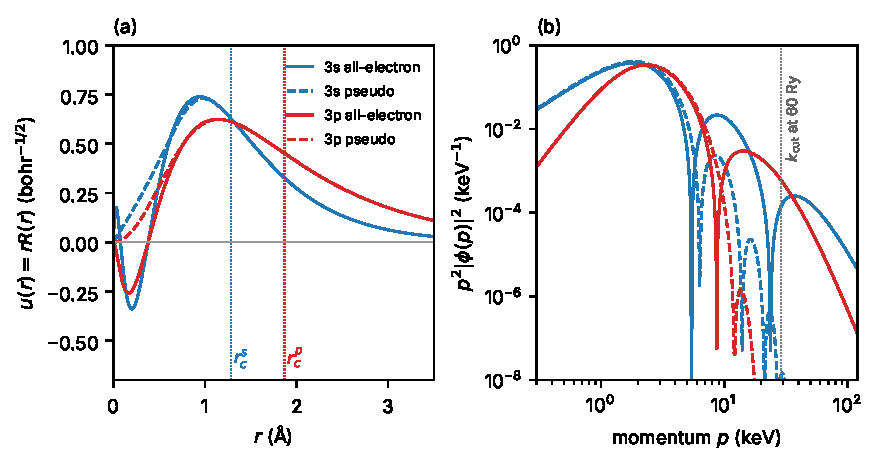
\includegraphics[width=\linewidth]{figures/ch03/fig3_9.pdf}
  \caption{The valence orbitals of the silicon atom near the nucleus, all-electron (solid) and pseudo (dashed), for $3s$ (blue) and $3p$ (red). (a)~Radial functions $u = rR$. The all-electron orbitals change sign at 0.08 and \SI{0.38}{\angstrom} ($3s$) and at \SI{0.38}{\angstrom} ($3p$) to stay orthogonal to the core; the pseudo-orbitals are nodeless inside the core radii $r_c$ (dotted). Outside them they equal the all-electron ones, and they carry the same charge inside. (b)~Momentum distributions $p^2|\phi(p)|^2$, normalized to $\int\dd p\,p^2|\phi|^2 = 1$; dotted, the plane-wave cutoff $k_{\mathrm{cut}} = \SI{28.9}{keV}$ at which the total energy of silicon converges (\SI{60}{Ry}). Free atom, all-electron calculation with the PBE functional, scalar-relativistic (mass--velocity and Darwin terms kept, spin--orbit coupling dropped), configuration $[\mathrm{Ne}]\,3s^23p^2$. The pseudopotential is a single-projector norm-conserving potential of the Troullier--Martins form~\cite{troullier1991efficient}, generated for this figure at the core radii of the SG15 potential of the plane-wave calculations, 1.27 and \SI{1.89}{\angstrom} for $s$ and $p$, to within \SI{0.02}{\angstrom}; it reproduces the all-electron eigenvalues. The SG15 potential has the same radii but a different shape inside them.}
  \label{fig:3-psae}
\end{figure}

\subsection{Projector augmented waves}

The core region that the pseudopotential discards can be restored. Outside the core spheres the pseudo-state is the true state, and inside each sphere the true state is fixed, up to a few coefficients, by the atom from which the pseudopotential was built. Bl\"ochl's \emph{projector-augmented-wave} (PAW) method makes the map from one to the other explicit and linear~\cite{blochl1994projector}. For each atom it uses three sets of functions, labeled by an index $j$ that collects the site, the angular momentum $lm$ and a reference energy. The \emph{all-electron partial waves} $\phi^{\mathrm{AE}}_j$ are solutions of the radial equation of the atom at the reference energies. The \emph{pseudo partial waves} $\phi^{\mathrm{PS}}_j$ are smooth functions that coincide with them outside the sphere. The \emph{projectors} $\tilde p_j$ are localized inside the sphere and dual to the pseudo partial waves, $\langle\tilde p_i|\phi^{\mathrm{PS}}_j\rangle = \delta_{ij}$. The pseudo partial waves are assumed complete for smooth functions inside the sphere, $\sum_j|\phi^{\mathrm{PS}}_j\rangle\langle\tilde p_j| = 1$ there. The all-electron state is then
\begin{equation}
  \csname ltx@label\endcsname{{eq:E.2-PAW}}%
  |\psi_{n\vect{k}}\rangle = |\tilde\psi_{n\vect{k}}\rangle + \sum_j\bigl(|\phi^{\mathrm{AE}}_j\rangle - |\phi^{\mathrm{PS}}_j\rangle\bigr)\langle\tilde p_j|\tilde\psi_{n\vect{k}}\rangle ,
  \label{eq:3.5-PAW}
\end{equation}
where $\tilde\psi_{n\vect{k}}$ is the smooth pseudo-state of the calculation. Outside the spheres the bracket vanishes and $\psi = \tilde\psi$. Inside a sphere, completeness lets us write the pseudo-state as its one-center expansion $\tilde\psi^1 = \sum_j\phi^{\mathrm{PS}}_j\langle\tilde p_j|\tilde\psi\rangle$, so that \cref{eq:3.5-PAW} subtracts it and puts in its place $\psi^1 = \sum_j\phi^{\mathrm{AE}}_j\langle\tilde p_j|\tilde\psi\rangle$, the same combination of all-electron partial waves. The nodes and the cusp come back with the $\phi^{\mathrm{AE}}_j$.

We can compute matrix elements without ever building $\psi$ on a fine grid. Write $\psi = \tilde\psi + \psi^1 - \tilde\psi^1$ for both states, and take an operator $A$ that is local, so that it does not connect the inside of a sphere with the outside. In a cross term such as $\langle\tilde\psi_m|A|\psi^1_n - \tilde\psi^1_n\rangle$ the difference lives inside the sphere, where $\tilde\psi_m = \tilde\psi^1_m$, and the cross term equals $\langle\tilde\psi^1_m|A|\psi^1_n - \tilde\psi^1_n\rangle$. Doing the same in the other cross term, the three terms that contain a difference combine into $\langle\psi^1_m|A|\psi^1_n\rangle - \langle\tilde\psi^1_m|A|\tilde\psi^1_n\rangle$, and
\begin{equation}
  \langle\psi_m|A|\psi_n\rangle = \langle\tilde\psi_m|A|\tilde\psi_n\rangle + \sum_{ij}\langle\tilde\psi_m|\tilde p_i\rangle\bigl(\langle\phi^{\mathrm{AE}}_i|A|\phi^{\mathrm{AE}}_j\rangle - \langle\phi^{\mathrm{PS}}_i|A|\phi^{\mathrm{PS}}_j\rangle\bigr)\langle\tilde p_j|\tilde\psi_n\rangle ,
  \label{eq:3.5-PAWop}
\end{equation}
with the partial-wave matrix elements taken inside the spheres. The smooth part is computed in plane waves at a modest cutoff. The rest is a sum of one-center terms, computed once for each species on a radial grid fine enough for the cusp.

\begin{keyresult}[All-electron density vertex]
With $A = \ee^{\ii\vect{q}\cdot\vect{r}}$ and $\vect{r} = \vect{\tau}_\kappa + \vect{x}$ in the sphere of atom $\kappa$ of the cell, \cref{eq:3.5-PAWop} gives the vertex of \cref{eq:3.2-rho} between all-electron states as
\begin{equation}
  \csname ltx@label\endcsname{{eq:E.2-rhoPAW}}%
  \rho_{mn}(\vect{k}, \vect{q}) = \langle\tilde\psi_{m,\vect{k}+\vect{q}}|\ee^{\ii\vect{q}\cdot\vect{r}}|\tilde\psi_{n\vect{k}}\rangle
  + \sum_\kappa\ee^{\ii\vect{q}\cdot\vect{\tau}_\kappa}\sum_{ij}\langle\tilde\psi_{m,\vect{k}+\vect{q}}|\tilde p_{\kappa i}\rangle\,\Delta_{\kappa,ij}(\vect{q})\,\langle\tilde p_{\kappa j}|\tilde\psi_{n\vect{k}}\rangle ,
  \label{eq:3.5-rhoAE}
\end{equation}
with the one-center matrix
\begin{equation}
  \Delta_{\kappa,ij}(\vect{q}) = \langle\phi^{\mathrm{AE}}_{\kappa i}|\ee^{\ii\vect{q}\cdot\vect{x}}|\phi^{\mathrm{AE}}_{\kappa j}\rangle - \langle\phi^{\mathrm{PS}}_{\kappa i}|\ee^{\ii\vect{q}\cdot\vect{x}}|\phi^{\mathrm{PS}}_{\kappa j}\rangle .
  \label{eq:E.2-onecentre}
\end{equation}
\end{keyresult}
Here we have written the atom index explicitly, $\tilde p_{\kappa i}$ for the projectors and $\phi_{\kappa i}$ for the partial waves of atom $\kappa$. The projections $\langle\tilde p_{\kappa j}|\tilde\psi_{n\vect{k}}\rangle$ are taken with the states normalized over one cell (\cref{app:A.5}). Every one of the $N$ cells contributes the same one-center terms by Bloch's theorem, each with weight $1/N$ for states normalized over the crystal, and the cell normalization adds them up; the phase is that of the atom in the reference cell. The plane wave about the nucleus expands into spherical Bessel functions $j_l(qx)$ times spherical harmonics (\cref{eq:C.3-planewave}), so each element of $\Delta_{\kappa,ij}$ is a sum of radial integrals of $j_l(qx)$ against products of partial waves, times Gaunt coefficients (integrals of three spherical harmonics). These are computed once per species and per $|q|$.

How large is the correction? Expand $\Delta_{\kappa,ij}(\vect{q})$ in $\vect{q}\cdot\vect{x}$. The zeroth-order term is the difference of overlaps inside the sphere. For partial waves that obey the generalized norm-conservation condition it vanishes; a PAW data set does not require that condition, and the term is then the charge that the smooth part lacks inside the sphere. The first-order term is a difference of dipole moments of partial-wave products, of relative size $qr_c$, weighted by the fraction of the state inside the sphere; the next is a quadrupole difference, of order $(qr_c)^2$. The pseudo vertex is accurate for $qr_c \ll 1$, below about \SI{1}{keV} for the silicon potential above, and the correction grows from there. Well above $q_{\mathrm{opt}}$ it is the whole answer, since the pseudo vertex has decayed. In between lies the range where most electron-recoil rates are decided. Griffin and coworkers computed the all-electron vertices of silicon and germanium in this way, from PAW calculations, and the valence-to-conduction rates for dark matter of \SI{1}{GeV}. For a heavy mediator, which weights large $q$, the reconstruction makes the differential rate much higher than the pseudo result at energy deposits above about \SI{15}{eV}, so that the rate integrated above a threshold is enhanced even for thresholds as low as about \SI{10}{eV}~\cite[Sects.~1 and~3.1]{griffin2021extended}. Together with the core states it raises it by more than an order of magnitude at higher thresholds, especially in germanium, while the light-mediator rate, dominated by small $q$, changes less~\cite[Sects.~3.1 and~4]{griffin2021extended}. A norm-conserving potential can be reconstructed with the same formula, using the partial waves of the atom from which it was built. The reconstruction is as good as its ingredients. It assumes a frozen core. It restores the core region only within the span of a few partial waves per channel, which is accurate near the reference energies and less so far above them. And it does not add the core states themselves, which are absent from the pseudopotential calculation. \Cref{app:E.7} gives the practice and its convergence.

\begin{workedexample}{The cutoff for momentum transfers up to 30 keV}\label{we:3-Ecut}
A momentum transfer $q = \SI{30}{keV}$ needs $2\mchi v_{\mathrm{max}} \ge q$, that is $\mchi \ge q/2v_{\mathrm{max}} = \SI{5.7}{MeV}$ for $v_{\mathrm{max}} = 2.650\times10^{-3}$, and it deposits at most $\omega = qv_{\mathrm{max}} = \SI{79.5}{eV}$. The final state lies at most \SI{79.5}{eV} above the valence-band maximum, or about \SI{92}{eV} above the bottom of the valence band. Its plane-wave components are concentrated below
\begin{equation*}
  p_f = [2m_e(\omega + E_{\mathrm{F}})]^{1/2} = (2\times\SI{0.511}{MeV}\times\SI{92}{eV})^{1/2} = \SI{9.7}{keV} .
\end{equation*}
By \cref{eq:3.5-Ecut}, the basis must hold the initial-state components up to $q + p_f = \SI{39.7}{keV}$:
\begin{equation*}
  E_{\mathrm{cut}} \gtrsim \frac{(\SI{39.7}{keV})^2}{2\times\SI{511}{keV}} = \SI{1.54}{keV} = \SI{113}{Ry} .
\end{equation*}
With $k_{\mathrm{cut}} = 10.6/a_0$ and the silicon cell of $270.3\,a_0^3$, in units of the Bohr radius $a_0 = \SI{0.529}{\angstrom}$, \cref{eq:E.1-npw} gives about 5500 plane waves per state, 2.6 times the 2121 at which the total energy has converged to \SI{0.1}{meV} per atom. The same estimate counts the bands below $\omega$: the free-electron states inside a sphere of radius $p_f$ number $\Omega p_f^3/6\pi^2 \approx 80$ per spin.

At \SI{60}{Ry}, $k_{\mathrm{cut}} = \SI{28.9}{keV}$. The vertex at \SI{30}{keV} is not zero there, since it vanishes identically only beyond $2k_{\mathrm{cut}} = \SI{58}{keV}$, but it lacks the initial-state components between 28.9 and \SI{39.7}{keV}. Raising the cutoff to \SI{113}{Ry} converges it, to the pseudo answer. In the atom of \cref{fig:3-psae}, the pseudo-orbitals carry less than $10^{-7}$ of their weight above \SI{30}{keV}, the all-electron orbitals 0.7 ($3s$) and \SI{0.4}{\percent} ($3p$): the converged pseudo vertex at \SI{30}{keV} misses almost all of the true one. Only the reconstruction \cref{eq:3.5-rhoAE} restores the tail, and the cutoff estimate applies to the reconstructed states. The silicon and germanium calculation of Griffin and coworkers meets these requirements: pseudo-states at a cutoff of \SI{1}{keV}, reconstructed all-electron states up to \SI{2}{keV}, which hold momentum components up to $(2m_e\times\SI{2}{keV})^{1/2} = \SI{45}{keV}$~\cite[Sect.~2.1]{griffin2021extended}.
\end{workedexample}

\subsection{Core and semicore states}

Below the valence bands of silicon lie the atomic shells $2p$, $2s$ and $1s$. Their binding energies relative to the valence-band maximum, measured by photoemission, are \SI{99.4}{eV} for $2p$ (the $2p_{3/2}$ level; $2p_{1/2}$ is at \SI{99.8}{eV}), \SI{150}{eV} for $2s$ and \SI{1839}{eV} for $1s$~\cite[Table~1-1]{williams2009electron}. Their radial densities peak at 0.21, 0.24 and \SI{0.038}{\angstrom} from the nucleus, against about \SI{1}{\angstrom} for the $3s$ and $3p$ valence orbitals. Half of the $2p$ electrons have momenta above \SI{14}{keV}, and half of the $1s$ electrons above \SI{37}{keV}; for the valence electrons the median is 2 to \SI{3}{keV}. These are free-atom numbers, from the all-electron calculation of \cref{fig:3-core}, but the core shells change little in the crystal. A pseudopotential calculation contains none of these states.

Whether they matter is decided by kinematics. An electron in a shell at depth $E_{\mathrm{core}}$ below the valence-band maximum needs at least $\omega = \Eg + E_{\mathrm{core}}$ to reach the conduction band. By \cref{eq:1.3-vmin}, a particle of mass $\mchi$ deposits $\omega$ at momentum transfer $q$ only if $\omega/q + q/2\mchi \le v_{\mathrm{max}}$. Since the second term is positive, the momentum transfer must exceed $\omega/v_{\mathrm{max}}$; minimizing the left-hand side over $q$, at $q = (2\mchi\omega)^{1/2}$, gives the threshold mass $2\omega/v_{\mathrm{max}}^2$ of \cref{eq:1.3-mmin}. With $v_{\mathrm{max}} = 2.650\times10^{-3}$, the silicon $2p$ shell needs $q \ge \SI{38}{keV}$ for any mass and opens at $\mchi = \SI{29}{MeV}$, where the only usable momentum transfer is $(2\mchi\omega)^{1/2} = 2\omega/v_{\mathrm{max}} = \SI{76}{keV}$. The $2s$ shell needs $q \ge \SI{57}{keV}$ and opens at \SI{43}{MeV}, with \SI{114}{keV} there, and the $1s$ shell opens above \SI{0.5}{GeV}. Below about \SI{29}{MeV}, dark matter scatters only on the four valence electrons of each silicon atom. Above, the $2p$ shell is reached through the tail of its momentum distribution: \SI{3}{\percent} of its weight lies above \SI{38}{keV}.

Germanium is different. Its $3d$ shell lies only \SI{29}{eV} below the valence-band maximum~\cite[Table~1-1]{williams2009electron}, with a radial density peaked at \SI{0.27}{\angstrom}. It needs $q \ge \SI{11}{keV}$ for any mass, \SI{22}{keV} at the threshold mass $\mchi = \SI{8.5}{MeV}$, and three quarters of its momentum distribution lies above \SI{11}{keV}. Ten electrons per atom, kinematically accessible to light dark matter and probed near the peak of their momentum distribution, are what the field calls a \emph{semicore} shell: too deep to bond, too shallow and too extended to be frozen without loss. A germanium pseudopotential can freeze it, with four valence electrons, or keep it in the valence, with fourteen and a higher cutoff (\cref{app:E.2}). Only the second choice puts the $3d$ states into the calculated response. For a heavy mediator, and once their large-momentum components are restored, the $3d$ electrons dominate the total rate of germanium for $\mchi \gtrsim \SI{30}{MeV}$ at a one-pair threshold~\cite[Sects.~1 and~3.3]{griffin2021extended}, a point to which \cref{sec:10.6} returns. The deeper shells, $3p$ and below in germanium and all core shells of silicon, are added as atomic orbitals arranged in Bloch sums (\cref{eq:E.7-core}).

\begin{figure}[tbp]
  \centering
  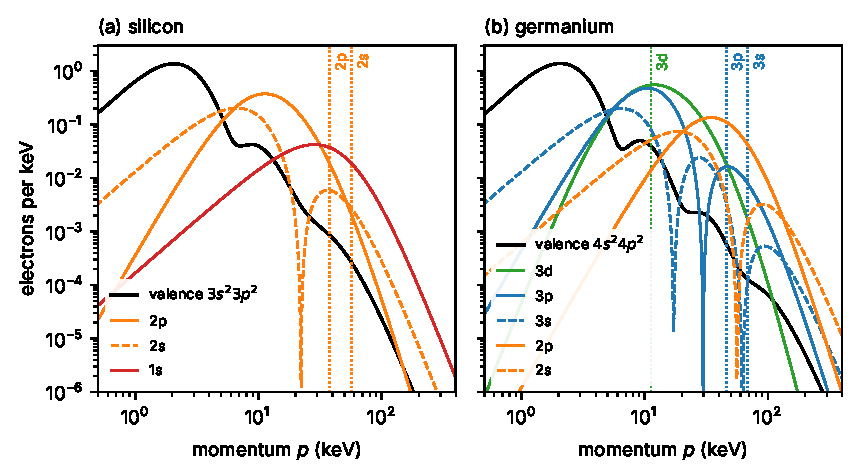
\includegraphics[width=\linewidth]{figures/ch03/fig3_10.pdf}
  \caption{How the electrons of each atomic shell are distributed in momentum, for (a)~silicon and (b)~germanium: electrons per keV of momentum magnitude, $N_{nl}\,p^2|\phi_{nl}(p)|^2$, with $N_{nl}$ the occupation of the shell and $\phi_{nl}$ the radial momentum-space orbital normalized to $\int\dd p\,p^2|\phi_{nl}|^2 = 1$. The orbitals are those of the free atoms, from an all-electron, scalar-relativistic calculation with the PBE functional (configurations $[\mathrm{Ne}]\,3s^23p^2$ and $[\mathrm{Ar}]\,3d^{10}4s^24p^2$; germanium $1s$, which opens above $q = \SI{4}{MeV}$, is not shown). Black: the valence shell. Dotted vertical lines: the smallest momentum transfer at which dark matter of any mass can lift an electron of the shell of the same color into the conduction band, $(\Eg + E_{\mathrm{core}})/v_{\mathrm{max}}$ (twice that at the threshold mass), with $v_{\mathrm{max}} = 2.650\times10^{-3}$, gaps of 1.17 and \SI{0.744}{eV} and measured binding energies relative to the valence-band maximum~\cite[Table~1-1]{williams2009electron}. Above about \SI{5}{keV} the core electrons outnumber the valence electrons in both atoms. The silicon $2p$ shell opens at \SI{38}{keV}, in the tail of its distribution; the germanium $3d$ shell opens at \SI{11}{keV}, near its peak.}
  \label{fig:3-core}
\end{figure}

\Cref{fig:3-core} also explains why the valence states need the core region. Above about \SI{5}{keV} the core electrons outnumber the valence electrons in both atoms, and at \SI{30}{keV} the silicon $2p$ shell holds forty times more weight per keV than the valence shell. What weight the valence shell has there comes from the inner lobes that keep it orthogonal to the core. These are the lobes that a pseudopotential removes and that \cref{eq:3.5-rhoAE} restores.

\subsection{Relativistic corrections}

A $1s$ electron of germanium moves at about $Z\alpha = 0.23$ of the speed of light, and the core electrons that a large momentum transfer probes are the fastest electrons of the atom. How large are the relativistic corrections to their states? For a single electron in the potential energy $U_1(\vect{r})$ of the nuclei and the other electrons, the Dirac equation $(\boldsymbol{\alpha}_{\mathrm{D}}\cdot\vect{p} + \beta_{\mathrm{D}}m_e + U_1)\psi = E\psi$ (\cref{app:C.15}) couples a large upper component $\psi_{\mathrm{A}}$ to a small lower one $\psi_{\mathrm{B}}$,
\begin{equation*}
  \boldsymbol{\sigma}\cdot\vect{p}\,\psi_{\mathrm{B}} = (\epsilon - U_1)\,\psi_{\mathrm{A}}, \qquad
  \boldsymbol{\sigma}\cdot\vect{p}\,\psi_{\mathrm{A}} = (2m_e + \epsilon - U_1)\,\psi_{\mathrm{B}} ,
\end{equation*}
with $\epsilon = E - m_e$ the energy without the rest mass. The second equation gives $\psi_{\mathrm{B}} = (2m_e + \epsilon - U_1)^{-1}\boldsymbol{\sigma}\cdot\vect{p}\,\psi_{\mathrm{A}}$. Wherever $|\epsilon - U_1| \ll 2m_e$, which fails within $Z\alpha/2m_e$ of a nucleus, we expand to first order, $\psi_{\mathrm{B}} \simeq (2m_e)^{-1}[1 - (\epsilon - U_1)/2m_e]\boldsymbol{\sigma}\cdot\vect{p}\,\psi_{\mathrm{A}}$, and insert it into the first equation. With $(\boldsymbol{\sigma}\cdot\vect{p})^2 = p^2$,
\begin{equation*}
  \Bigl[\frac{p^2}{2m_e} + U_1 - \frac{\boldsymbol{\sigma}\cdot\vect{p}\,(\epsilon - U_1)\,\boldsymbol{\sigma}\cdot\vect{p}}{4m_e^2}\Bigr]\psi_{\mathrm{A}} = \epsilon\psi_{\mathrm{A}} .
\end{equation*}
This is not yet a Schr\"odinger equation, since the energy appears on both sides and $\psi_{\mathrm{A}}$ is not normalized: the probability is $\int(|\psi_{\mathrm{A}}|^2 + |\psi_{\mathrm{B}}|^2) = \int\psi_{\mathrm{A}}^\dagger(1 + p^2/4m_e^2)\psi_{\mathrm{A}}$ to this order. The normalized two-component state is $\Phi = (1 + p^2/8m_e^2)\psi_{\mathrm{A}}$. We substitute $\psi_{\mathrm{A}} = (1 - p^2/8m_e^2)\Phi$ and multiply the equation from the left by $1 - p^2/8m_e^2$, keeping terms to order $1/m_e^2$ relative to $p^2/2m_e$. The kinetic term becomes $p^2/2m_e - p^4/8m_e^3$; the potential becomes $U_1 - (p^2U_1 + U_1p^2)/8m_e^2$; the term $-\epsilon p^2/4m_e^2$ on the left cancels the same term that the right-hand side, $\epsilon(1 - p^2/4m_e^2)\Phi$, acquires. What remains is
\begin{equation*}
  H\Phi = \Bigl[\frac{p^2}{2m_e} + U_1 - \frac{p^4}{8m_e^3} - \frac{p^2U_1 + U_1p^2}{8m_e^2} + \frac{\boldsymbol{\sigma}\cdot\vect{p}\,U_1\,\boldsymbol{\sigma}\cdot\vect{p}}{4m_e^2}\Bigr]\Phi = \epsilon\Phi .
\end{equation*}
The last two terms simplify with $[\vect{p}, U_1] = -\ii\nabla U_1$. Moving $\vect{p}$ to the right, $p^2U_1 = U_1p^2 - 2\ii\nabla U_1\cdot\vect{p} - \nabla^2U_1$, and with $(\boldsymbol{\sigma}\cdot\vect{a})(\boldsymbol{\sigma}\cdot\vect{b}) = \vect{a}\cdot\vect{b} + \ii\boldsymbol{\sigma}\cdot(\vect{a}\times\vect{b})$, $\boldsymbol{\sigma}\cdot\vect{p}\,U_1\,\boldsymbol{\sigma}\cdot\vect{p} = U_1p^2 - \ii\nabla U_1\cdot\vect{p} + \boldsymbol{\sigma}\cdot(\nabla U_1\times\vect{p})$. The terms in $U_1p^2$ and in $\nabla U_1\cdot\vect{p}$ cancel between the two, and
\begin{equation}
  H = \frac{p^2}{2m_e} + U_1 \underbrace{{}- \frac{p^4}{8m_e^3}}_{H_{\mathrm{mv}}} \underbrace{{}+ \frac{\nabla^2U_1}{8m_e^2}}_{H_{\mathrm{Dar}}} \underbrace{{}+ \frac{\boldsymbol{\sigma}\cdot(\nabla U_1\times\vect{p})}{4m_e^2}}_{H_{\mathrm{so}}} .
  \label{eq:3.5-HBP}
\end{equation}
The \emph{mass--velocity} term $H_{\mathrm{mv}}$ is the next term of the expansion of $(p^2 + m_e^2)^{1/2}$: a fast electron is heavier. The \emph{Darwin} term $H_{\mathrm{Dar}}$ smears the potential over the Compton wavelength $1/m_e$. For the nuclear attraction $-Z\alpha/r$ it is the contact term $(\pi Z\alpha/2m_e^2)\,\delta^3(\vect{r})$, felt only by $s$ electrons. In a central potential $\nabla U_1\times\vect{p} = r^{-1}(\dd U_1/\dd r)\vect{L}$, and with $\boldsymbol{\sigma} = 2\vect{S}$ the last term is the spin--orbit coupling \cref{eq:3.3-HSO}, now with its coefficient, including the Thomas factor, derived rather than quoted. The Foldy--Wouthuysen transformation reaches the same three operators by a unitary transformation, systematically to any order, and also gives the corresponding correction to $\ee^{\ii\vect{q}\cdot\vect{r}}$ (\cref{app:C.15}).

The size of each term follows from the velocity. For a hydrogen-like orbital, the virial theorem makes the mean kinetic energy equal to the binding energy, $\langle p^2\rangle/2m_e = (Z\alpha)^2m_e/2n^2$, so that $\langle v^2\rangle = (Z\alpha/n)^2$. The mass--velocity and Darwin terms are of relative order $\langle v^2\rangle$, and so is the change of the wavefunction near the nucleus. For $1s$ both can be evaluated. Since $p^2/2m_e = \epsilon - U_1$ for the eigenstate, $\langle p^4\rangle = 4m_e^2\langle(\epsilon - U_1)^2\rangle$. With $\epsilon = -(Z\alpha)^2m_e/2$, $\langle U_1\rangle = 2\epsilon$ and $\langle U_1^2\rangle = (Z\alpha)^2\langle r^{-2}\rangle = 2(Z\alpha)^4m_e^2$, this is $5(Z\alpha)^4m_e^4$, and $\langle H_{\mathrm{mv}}\rangle = -\tfrac58(Z\alpha)^4m_e$. The Darwin term is $(\pi Z\alpha/2m_e^2)|\psi_{1s}(0)|^2 = +\tfrac12(Z\alpha)^4m_e$, with $|\psi_{1s}(0)|^2 = (Z\alpha m_e)^3/\pi$. Each is a fraction of order $(Z\alpha)^2$ of the binding energy $(Z\alpha)^2m_e/2$, and they nearly cancel: their sum deepens the level by a quarter of $(Z\alpha)^2$ of its binding energy, the $1s$ term of the Dirac fine-structure formula. Relativistic effects are therefore of order $(Z\alpha)^2$ in the state and of order $(Z\alpha)^2/4$ in the energy of a $1s$ shell.

In practice, pseudopotentials and PAW data sets are generated from \emph{scalar-relativistic} atoms~\cite{koelling1977technique}: the mass--velocity and Darwin terms are kept in the radial equation, which stays independent of spin, and spin--orbit coupling is dropped. The core-region shape of the valence states, and the partial waves of \cref{eq:3.5-PAW}, then contain the leading relativistic contraction, and a reconstructed vertex inherits it. Spin--orbit coupling is added, when needed, with fully relativistic potentials (\cref{app:E.1}).

For the core shells, spin--orbit coupling is the visible effect. A shell with $l \ge 1$ splits into $j = l \pm \tfrac12$, by $(l + \tfrac12)\xi_{\mathrm{SO}}$, the $p$ splitting $\tfrac32\xi_{\mathrm{SO}}$ of \cref{sec:3.3} generalized. Near the nucleus $r^{-1}\dd U_1/\dd r \simeq Z\alpha/r^3$, and for an inner shell, which lives there, $\langle r^{-3}\rangle$ grows as $Z^3$, so that $\xi_{\mathrm{SO}}$ grows as $Z^4$. The hydrogen-like $2p$ splitting $(Z\alpha)^4m_e/32$ of \cref{sec:3.3} is an upper bound for a real atom, in which the outer part of the orbital sees a screened charge: it would be \SI{1.7}{eV} for silicon and \SI{47}{eV} for germanium. A Dirac--Kohn--Sham calculation of the atoms yields 0.65 and \SI{31.9}{eV}, and the measured germanium $2p$ doublet, at 1217.0 and \SI{1248.1}{eV}, is split by \SI{31.1}{eV}~\cite[Table~1-1]{williams2009electron}. A core edge is therefore a doublet. In the $2p$ edge of silicon the two components lie a few tenths of an eV apart, while those of the germanium $3d$ edge, the one light dark matter reaches, lie \SI{0.6}{eV} apart, with the statistical weights $4:6$ of $3d_{3/2}$ and $3d_{5/2}$.

\begin{workedexample}{Relativistic corrections for silicon and germanium core states}\label{we:3-Zalpha}
With $\alpha = 1/137.036$, the squared velocity of a $1s$ electron is
\begin{gather*}
  (Z\alpha)^2 = \Bigl(\frac{14}{137.036}\Bigr)^2 = 0.0104 \quad\text{(silicon)}, \\
  (Z\alpha)^2 = \Bigl(\frac{32}{137.036}\Bigr)^2 = 0.0545 \quad\text{(germanium)}.
\end{gather*}
These are the relative sizes of the mass--velocity and Darwin terms, and of the relativistic change of the $1s$ orbitals: \SI{1}{\percent} in silicon, \SI{5}{\percent} in germanium. The binding energy shifts by $(Z\alpha)^2/4$ of itself, 0.26 and \SI{1.36}{\percent}. All-electron calculations of the free atoms with the PBE functional, with and without the mass--velocity and Darwin terms, check this. The $1s$ level of silicon moves from $-1781.2$ to \SI{-1785.9}{eV}, by \SI{0.26}{\percent}, and that of germanium from $-10\,803$ to \SI{-10961}{eV}, by \SI{1.46}{\percent}. The screening of the nucleus by the other electrons changes the binding energies, but hardly the ratio.

The germanium $3d$ shell is not hydrogen-like, and we estimate an effective charge from its size. A hydrogen-like orbital has $\langle r\rangle = [3n^2 - l(l + 1)]/2Z_{\mathrm{eff}}$ in bohr, $10.5/Z_{\mathrm{eff}}$ for $3d$. The atomic calculation gives $\langle r\rangle = 0.737$ bohr, so $Z_{\mathrm{eff}} = 14.2$, and
\begin{equation*}
  \langle v^2\rangle = \Bigl(\frac{Z_{\mathrm{eff}}\alpha}{n}\Bigr)^2 = \Bigl(\frac{14.2}{3\times137.036}\Bigr)^2 = 1.2\times10^{-3} .
\end{equation*}
The direct relativistic correction to the $3d$ states is about \SI{0.1}{\percent}. The atomic calculation shows a larger, indirect effect of the opposite sign: the scalar-relativistic Kohn--Sham $3d$ level lies at \SI{-29.31}{eV} instead of \SI{-30.15}{eV}, \SI{2.8}{\percent} less bound. The $s$ and $p$ shells inside it contract, screen the nucleus more strongly, and push the $3d$ level up. Spin--orbit coupling splits the level by \SI{0.59}{eV} in the Dirac--Kohn--Sham atom, against the measured \SI{0.6}{eV}, or \SI{2}{\percent} of the binding energy~\cite[Table~1-1]{williams2009electron}.

Dark matter lighter than \SI{0.3}{GeV} reaches every shell except silicon $1s$ and germanium $2p$ and below. Each shell it reaches needs relativistic corrections of at most a few percent in energy, and less in its states. A scalar-relativistic pseudopotential or PAW data set includes the leading part, and the spin--orbit doublet of the $3d$ edge is the one correction that a spectrum resolves.
\end{workedexample}
